\documentclass{article}
% Chinese
% \documentclass[UTF8, nofonts, mathptmx, 12pt, onecolumn]{article}
% \usepackage{xeCJK}
% \setCJKmainfont{SimSun}
\usepackage{amsmath}
\usepackage{amsfonts}
\usepackage{amssymb}
\usepackage{wasysym}
% \usepackage{ctex}
\usepackage{graphicx}
\usepackage{float}
\usepackage{geometry}
\geometry{a4paper,scale=0.8}
\usepackage{caption}
\usepackage{subcaption}
% \newcommand{\oiint}{\mathop{{\int\!\!\!\!\!\int}\mkern-21mu \bigcirc} {}}
\newcommand*{\dif}{\mathop{}\!\mathrm{d}}
\newcommand*{\md}{\mathop{}\!\mathrm{d}}
\newcommand*{\me}{\mathrm{e}}

% \usepackage{parskip}
% \setlength{\parindent}{0cm}

\usepackage{bm}
\let\Oldmathbf\mathbf
\renewcommand{\mathbf}[1]{\boldsymbol{\Oldmathbf{#1}}}
\let\eqnarray\align

\author{Xiping Hu}
\usepackage{authblk}
\author{Xiping Hu}
\affil{http://thehxp.tech/}
\title{Homework for Chapter 2}

\begin{document}
\maketitle

\begin{figure}[H]
  \centering
  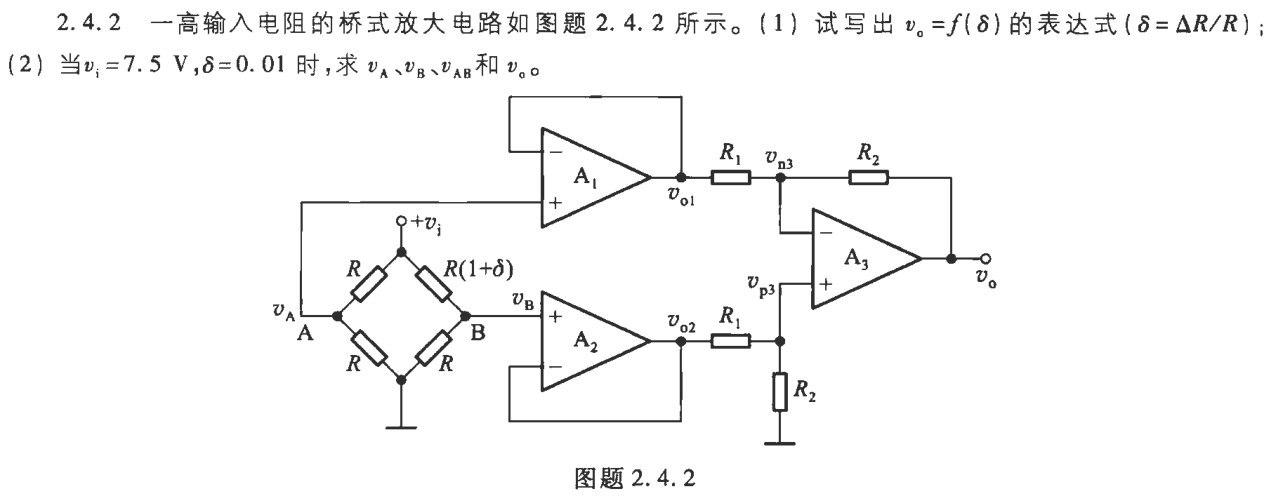
\includegraphics[width=0.9\linewidth]{figures/Problem2-1}
  \label{fig:}
\end{figure}

\paragraph{Solution}

According to the "Virtual-Open-Circuited" theory, the current will not either go left at node A nor go right at node B

\begin{equation*}
  \begin{aligned}
    v_A &= \dfrac{v_i}{2} \\
    v_B &= \dfrac{v_i}{2 + \delta} 
  \end{aligned}
\end{equation*}

For the 2 operational amplifiers $A_1$ and $A_2$ 

\begin{equation*}
  \begin{aligned}
    v_{o2} &= v_B = \dfrac{v_i}{2 + \delta} \\
    v_{o1} &= v_A = \dfrac{v_i}{2}
  \end{aligned}
\end{equation*}

Then we can calculate the input voltage of operational amplifier $A_3$

\begin{equation*}
  \begin{aligned}
    v_{p3} &= \dfrac{R_2}{R_1 + R_2} v_{o2} =  \dfrac{R_2}{R_1 + R_2} \dfrac{v_i}{2 + \delta} \\
    v_{n3} &= v_{p3} = \dfrac{R_2}{R_1 + R_2} \dfrac{v_i}{2 + \delta}
  \end{aligned}
\end{equation*}

Since $A_3$ is an ideal operational amplifier

\begin{equation*}
  \begin{aligned}
    I_{R1} = I_{R2} = \dfrac{v_{o1} - v_{n3}}{R_1} =  \left( \dfrac{v_i}{2} - \dfrac{R_2}{R_1 + R_2} \dfrac{v_i}{2 + \delta} \right) \dfrac{1}{R_1} 
  \end{aligned}
\end{equation*}

\begin{equation*}
  \begin{aligned}
    v_{n3} - v_o = I_{R1} R_2 = \dfrac{v_{o1} - v_{n3}}{R_1} =  \left( \dfrac{v_i}{2} - \dfrac{R_2}{R_1 + R_2} \dfrac{v_i}{2 + \delta} \right) \dfrac{R_2}{R_1} 
  \end{aligned}
\end{equation*}

Finally, we get

\begin{equation*}
  \begin{aligned}
    v_o &= \dfrac{R_2}{R_1 + R_2} \dfrac{v_i}{2 + \delta} - \left( \dfrac{v_i}{2} - \dfrac{R_2}{R_1 + R_2} \dfrac{v_i}{2 + \delta} \right) \dfrac{R_2}{R_1} \\
    &= \left( \dfrac{R_1}{R_1 + R_2} \dfrac{v_i}{2 + \delta} - \dfrac{v_i}{2} + \dfrac{R_2}{R_1 + R_2} \dfrac{v_i}{2 + \delta} \right) \dfrac{R_2}{R_1} \\
    &= \dfrac{R_2}{R_1} \left( - \dfrac{1}{2} + \dfrac{1}{2 + \delta} \right) v_i \\
    &= \dfrac{R_2}{R_1} \left( \dfrac{- \delta}{4 + 2 \delta}  \right) v_{i} 
  \end{aligned}
\end{equation*}

When $v_i = 7.5 \  \mathrm{V}$, $\delta = 0.01$

\begin{equation*}
  \begin{aligned}
    v_o = - 0.01866 \times \dfrac{R_2}{R_1} 
  \end{aligned}
\end{equation*}




\end{document}